\subsection{Элементы физики твердого тела}

\subsubsection{Трансляционная симметрия --  определение, примеры объектов с трансляционной симметрией}

см. Алексеев экзамен \#2

\subsubsection{Функция распределения для свободных электронов (вывод). Связь энергии Ферми и концентрации электронов}
\label{sec:free-elecs}

Будем рассматривать металл как потенциальный ящик с абсолютно непроницаемыми стенками, в 
котором находятся электроны, не взаимодействующие между собой. Рассмотрим число квантовых состояний 
$N_E$, энергия которых меньше $E$ ($l_i$ -- размер коробки по $i$-ой координате):
\[
  E_{n_1, n_2, n_3} = \dfrac{\pi^2 \hbar^2}{2 m_e} \left(
    \left( \dfrac{n_1}{l_1} \right)^2 +
    \left( \dfrac{n_2}{l_2} \right)^2 +
    \left( \dfrac{n_3}{l_3} \right)^2 \right) < E
\]
обозначая: $V = l_1 l_2 l_3 = l_0^3$, $\alpha_i = \dfrac{l_i}{l_0}$, получаем:
\[
  \dfrac{\pi^2 \hbar^2}{2 m_e l_0^3} \left(
    \left( \dfrac{n_1}{\alpha_1} \right)^2 +
    \left( \dfrac{n_2}{\alpha_2} \right)^2 +
    \left( \dfrac{n_3}{\alpha_3} \right)^2 \right) < E
\]
обозначим $E_0 = \dfrac{\pi^2 \hbar^2}{2 m_e l_0^3}$, $\varepsilon = \dfrac{E}{E_0}$:
\[
  \dfrac{1}{\varepsilon} \left(
    \left( \dfrac{n_1}{\alpha_1} \right)^2 +
    \left( \dfrac{n_2}{\alpha_2} \right)^2 +
    \left( \dfrac{n_3}{\alpha_3} \right)^2\right) < 1
  \Leftrightarrow
  \left( \dfrac{n_1}{\alpha_1 \sqrt{\varepsilon}} \right)^2 +
    \left( \dfrac{n_2}{\alpha_2 \sqrt{\varepsilon}} \right)^2 +
    \left( \dfrac{n_3}{\alpha_3 \sqrt{\varepsilon}} \right)^2 < 1
\]
Таким образом, приходим к тому, что нужно найти объём в пространстве квантовых чисел
(квазинепрерывном), это уравнение эллипса, поэтому объем равен 1/8 части объёма эллипса
(учитывая то, что каждое кв число больше 0):
\[
  \Omega_E = \dfrac{1}{8} \dfrac{4}{3} \pi (\sqrt{\varepsilon})^3 \alpha_1 \alpha_2 \alpha_3
  = \dfrac{1}{6} \pi \varepsilon^{3/2}.
  \Rightarrow
  N_\text{Я} = \dfrac{1}{6} \pi \varepsilon^{3/2}
  = \dfrac{1}{6} \pi E^{3/2} \left( \dfrac{2 m_e l_0^3}{3 \pi^2 \hbar^2} \right)^{3/2}
  = \dfrac{\sqrt{2} m_e^{3/2}}{3 \pi^2 \hbar^3} E^{3/2} V
\]
с учётом спина:
\[
  N_E = 2 N_\text{Я} = \dfrac{2 \sqrt{2} m_e^{3/2}}{3 \pi^2 \hbar^3} E^{3/2} V 
\]
перейдём к концентрации:
\[
  \tilde n_E = \dfrac{N_E}{V} = \dfrac{2 \sqrt{2} m_e^{3/2}}{3 \pi^2 \hbar^3} E^{3/2}.
\]
Это количество состояний, для которых энергия меньше $E$, для получения концентрации состояний в
отрезке $[E, E+\Delta E]$, продифференцируем это:
\[
  dn_E = \dfrac{\sqrt{2} m_e^{3/2}}{\pi^2 \hbar^3} \sqrt{E} dE
  \Rightarrow
  g(E) = \dfrac{d\tilde n_E}{dE} = \dfrac{\sqrt{2} m_e^{3/2}}{\pi^2 \hbar^3} \sqrt{E}
\]

Распределение свободных электронов по энергиям:
\[
  dn_E = f_\text{Ф-Д} (E) d\tilde N_E = \dfrac{\sqrt{2} m_e^{3/2}}{\pi^2 \hbar^3} \dfrac{\sqrt{E}}{e^{\dfrac{E-E_F}{kT}} + 1}
\]

Можно чуть проанализировать эту формулу, например, в предельном случае $T \to 0$, распределение
Ферми-Дирака представляет собой просто ступеньку, а значит для энергий $E > E_F$ получим 0, то
есть нет таких электронов, а все состояния $E < E_F$ заполнены. Графический анализ на рисунке \ref{fig:free-electrons}.

\begin{figure}[H]
  \centering
  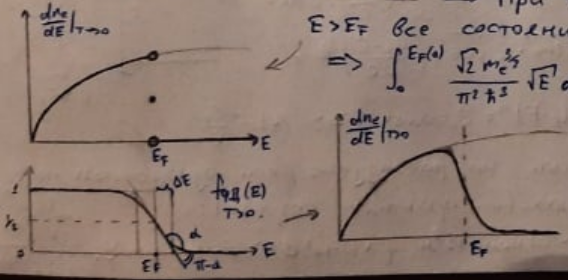
\includegraphics[width=.9\linewidth]{img/oral-04/oral-04-distribution-of-free-electrons.png}
  \caption{Графики распределения свободных электронов.
  График распределения при $T \to 0$ (слева-сверху).
  График распределения при увеличении температуры (справа).
  Графическое описания нахождения размытия уровня Ферми (слева-снизу)}
  \label{fig:free-electrons}
\end{figure}

\subsubsection{Оценка величины "размытия уровня Ферми" при $0 < kT \ll E_F$}

Продолжением анализа прошлого результата (про распределение свободных электронов) является анализ
того, что происходит с распределением при увеличении температуры. Так как при выполненом соотношении
$0 < kT \ll E_F$ график слабо отличается от графика при $T \to 0$ вне некоторого интервала
шириной $\Delta E$ вокруг точки $E_F$, ширину этого интервала можно оценить графически:
провести касательную к графику в точке $E_F$ (учитывая, что $dn_E / dE (E_F) = 1/2$):
\[
  |\tg (\pi - \alpha)| = \dfrac{1/2}{\Delta E} = \dfrac{1}{2 \Delta E}, 
  |\tg (\pi - \alpha)| = |\tg \alpha| = \left( \dfrac{d f_\text{Ф-Д}}{dE} \right)_{E = E_F} = \dfrac{1}{4kT}
  \Rightarrow \Delta E \approx 2kT
\]

\subsubsection{Влияние напряженности электрического поля на процесс ТЭЭ}
\label{sec:o244}
Cм. раздел \ref{sec:w7}. Если прикладывать напряжение между катодом и анодом, то работа
выхода металла будет смещаться. Причём приложим его в таком направлении, что
электроны будут притягиваться к аноду. Это приведёт к уменьшению $A_B$. Ключевым вопросом
является то, насколько изменится работа выхода внутри некоторого электрического поля.
Рассмотрим электрон, который вылетел с поверхности металла. Сила, с которой металл
притягивает его назад может быть найдена с помощью метода изображений. Согласно этому
методу, сила, действующая на заряженную частицу со стороны проводящей поверхности на расстоянии $x$,
равна силе, действующей между этой частицей и такой же, но с другим знаком на расстоянии $2x$:
$F_\text{из} = - \dfrac{k e^2}{(2x)^2}$. Потенциальная энергия такого
взаимодействия будет равна:
\[
  U_\text{из} = \int_x^{+\infty} F_\text{из} (t) \, dt
  =  - \dfrac{k e^2}{4 x}
\]
приложим теперь внешнее электрическое поле с напряженностью $\vec{\varepsilon}$, способствующее
выходу электронов из металла: $U_e = - e \varepsilon x, \vec{F} = - e \vec{\varepsilon}$.
Тогда общий потенциал:
\[
  U(x) = U_0 - e \varepsilon x - \dfrac{k e^2}{4 x} = U_0 - \alpha x - \dfrac{\beta}{x}.
\]
найдём максимум потенциальной энергии:
\[
  \dfrac{\partial U}{\partial x} (x_0) = 0 \Leftrightarrow x_0 = \sqrt{\dfrac{\beta}{\alpha}},
\]
и тогда значение изменения работы выхода будет:
$\Delta A_B = U_0 - U(x_0) = 2 \sqrt{\alpha \beta} = e^{3/2} k^{1/2} \varepsilon^{1/2}$,
тогда ток насыщения:
\[
  J_{x, \varepsilon}
  = const T^2 e^{-\dfrac{A_B - \Delta A_B}{kT}}
  = const T^2 e^{-\dfrac{A_B}{kT}} e^{ \dfrac{e^{3/2} k^{1/2} \varepsilon^{1/2}}{kT} }
  \Leftrightarrow
  \ln J_{x, \varepsilon}
  = const_1 + const_2 \varepsilon^{1/2}
\]
то есть ток будет увеличиваться и работа выхода будет уменьшаться.
На рисунке \ref{fig:shottki} приведена графическая иллюстрация.

\begin{figure}[H]
  \centering
  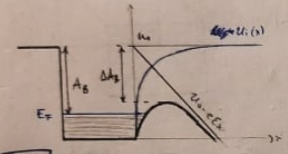
\includegraphics[width=.9\linewidth]{img/oral-04/Shottki.png}
  \caption{График потенциала $U_i$ до приложения внешнего поля (строго монотонный график,
  асимптота к которому горизонтальная линия);
  график потенциала после приложения внешнего поля (горка, асимптота -- прямая наклонная линия $U_0 = - e \varepsilon x$)}
  \label{fig:shottki}
\end{figure}


\subsubsection{Особенности зонной структуры легированных полупроводников. Оценка величины <<энергии ионизации>> примесных уровней}

\textit{Легирование полупроводников} — внедрение небольших количеств примесей или структурных дефектов с целью контролируемого изменения электрических свойств полупроводника.

см. Алексеев экзамен \#4
Примеси бывают разные. Они приводят к появлению избыточного количества или сво-
бодных электронов, или дырок. Их называют соответственно \textit{донорными} примесями (отдаю-
щими электроны) или \textit{акцепторными} примесями (забирающими электроны).

Соответственно легированные проводники бывают двух типов в зависимости от примесей, которые в них добавили:
\paragraph{Донорные полупроводники} 
В таких п/п избыток положительных свободных носителей заряда.

Донорные полупроводники -- получаются при добавлении в полупроводник элементов, от которых легко <<отрывается>> электрон.

Электроны в \textit{донорном} полупроводнике принято называть \textit{основными носителями заряда}, а дырки -- \textit{неосновными носителями заряда}.
\begin{figure}[H]
	\begin{minipage}{0.48\textwidth}
		\centering
		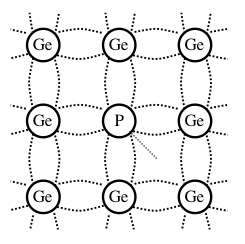
\includegraphics[width=0.7\linewidth]{img/oral-04/donor_poluprovodnik}
		\caption{Пример донорного полупроводника}
		\label{fig:donorpoluprovodnik}
	\end{minipage}\hfill
	\begin{minipage}{0.48\textwidth}
		\centering
		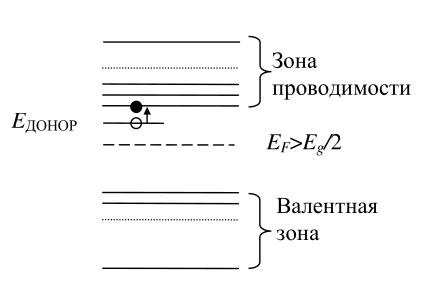
\includegraphics[width=\linewidth]{img/oral-04/donor_poluprovodnik1_energy}
		\caption{Энергетические уровни донорнрго полупроводника}
		\label{fig:donorpoluprovodnik1energy}
	\end{minipage}
\end{figure}
С точки зрения зонной теории наличие «легко отрывающихся» электронов соответствует появлению в запрещенной зоне донорных уровней энергии вблизи нижнего края зоны проводимости.

Уровень Ферми в донорном полупроводнике смещается вверх по шкале энергии, причем это смещение больше при низких температурах, когда концентрация свободных электронов значительно превышает число дырок. При повышении температуры, когда донорный характер полупроводника становится все менее и менее выраженным, уровень Ферми смещается в среднюю часть запрещенной зоны, как в беспримесном полупроводнике.
	
\paragraph{Акцепторные (дырочные, p-типа) полупроводники}
Получаются при добавлении в полупроводник элементов, которые легко <<отбирают>> электрон у атомов полупроводника. 
В таком случае в кристалле образуется избыток дырок.

Дырки в \textit{акцепторном} полупроводнике принято называть \textit{основными носителями}, а электроны - \textit{неосновными}.
\begin{figure}[H]
	\begin{minipage}{0.48\textwidth}
		\centering
		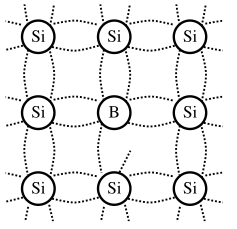
\includegraphics[width=0.7\linewidth]{img/oral-04/acceptor_poluprovodnik}
		\caption{Пример акцепторного полупроводника}
		\label{fig:acceptorpoluprovodnik}
	\end{minipage}\hfill
	\begin{minipage}{0.48\textwidth}
		\centering
		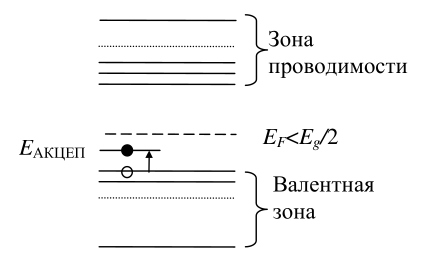
\includegraphics[width=\linewidth]{img/oral-04/acceptor_poluprovodnik1_energy}
		\caption{Энергетические уровни акцепторного полупроводника}
		\label{fig:acceptorpoluprovodnik1energy}
	\end{minipage}
\end{figure}

На языке зонной теории переход электрона из полноценной ковалентной связи в связь с недостающим электроном соответствует появлению в запрещенной зоне акцепторных уровней вблизи нижнего края зоны проводимости. Электрону для такого перехода из валентной зоны на акцепторный уровень требуется меньше энергии, чем для перехода из валентной зоны в зону проводимости, то есть для <<полного ухода>> электрона из ковалентной связи.

Уровень Ферми в акцепторном полупроводнике смещается вниз по шкале энергии, причем это смещение больше при низких температурах, когда концентрация дырок значительно превышает концентрацию свободных электронов. При повышении температуры, когда акцепторный характер полупроводника становится все менее и менее выраженным, уровень Ферми смещается в среднюю часть запрещенной зоны, как в беспримесном полупроводнике.

\paragraph{Энергия ионизации} --- энергия, которая необходимая для освобождения примесного электрона или дырки из примесного уровня. 

Для донорного полупроводника она отсчитывается от дна зоны проводимости до примесного уровня, а для акцепторного - от потолка валентной зоны по примесного уровня (см. Рис. \ref{fig:donorpoluprovodnik1energy} и \ref{fig:acceptorpoluprovodnik1energy}).

По значении энергии ионизации примесь делится на мелкую и глубокую. Если энергия ионизации примеси близка к половине ширины запрещенной зоны, то такую примесь называют глубокой. Если энергия ионизации примеси близка к уровню разрешенной зоны (реально меньше 0,1-0,05 еВ), то такую примесь называют мелкой. Чем больше энергия ионизации примеси, тем при той же температуре меньше концентрация свободных носителей заряда.

\subsubsection{Строение p-n перехода. Распределение объемного заряда, концетраций дырок и электронов, электрического потенциала. Вывод формулы Шокли}

$p-n$ нереходом называют тонкий слой, образующийся в месте контакта двух областей полупроводников
акцепторного и донорного типов. С одной стороны от перехода будет область $p$ типа, в которой
основным носителем заряда будут дырки, с другой стороны -- область $n$ типа, в которой основными
носителями заряда будут электроны. В области контакта полупроводников носители заряда будут
проходить через переход, вызывая <<рекомбинацию>> -- то есть взаимное <<уничтожение>> электрона и дырки.
За счёт этого вблизи границы концентрация обоих носителей близка к нулю.

Из-за распределения зарядов примесных ионов в зоне контакта возникает контактное электрическое поле,
которое "противодействует" переходу основных носителей через границу контакта. Это приводит к возникновению потенциального барьера высоты $U_0$, кроме того, подключённый источник гапряжения изменяет высоту потенциального барьера: повышает, если минус источника подключён к p-области.

В равновесном состояниии $j_\text{ОСН} = j_\text{НЕОСН}$, $j_\text{ОСН} = j_0 \cdot e^{-\dfrac{U_0}{kT}}$, а полный ток $j = j_\text{ОСН} - j_\text{НЕОСН} = 0$.

Если прикладывается напряжение $V>0$, то $j_\text{ОСН} = j_0 \cdot e^{-\dfrac{U_0-eV}{kT}}$, следовательно, $j = j_\text{ОСН} - j_\text{НЕОСН} = j_0 e^{-\dfrac{U_0-eV}{kT}} - j_0 \cdot e^{-\dfrac{U_0}{kT}} = j(T) \cdot \left( e^{\dfrac{eV}{kT}} - 1 \right) $ - формула Шокли.

\subsubsection{Эффект Холла в полупроводнике с двумя типами носителей заряда}

Рассмотрим полупроводник, находящийся в магнитном поле $\vec{B}$ и в электрическом поле
$\vec{E}_{||}$.  Концентрации и подвижности носителей зарядов обозначим $n_e, n_h, \mu_e, \mu_h$.
Скорость дрейфа обозначим $\vec{v}_d$. Для скорости дрейфа раннее (вопрос 10, равенство
\eqref{write:10:v_d}) было получено соотношение $\vec{v}_d = \mu \vec{E}$.

\begin{figure}[H]
  \label{oral04:halleffect}
  \centering
  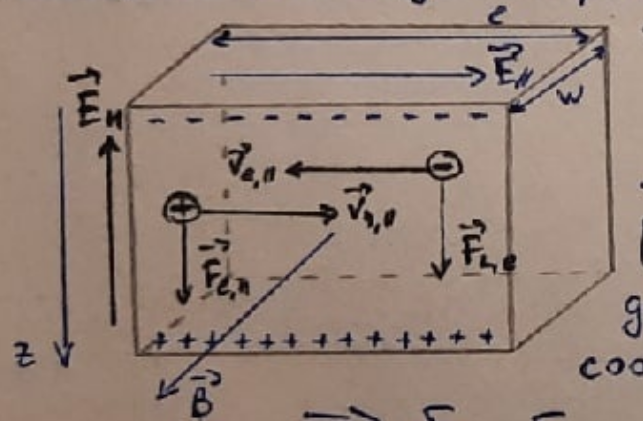
\includegraphics[width=0.9\linewidth]{img/oral-04/hall-effect.png}
  \caption{Иллюстрация эффекта Холла}
\end{figure}

На заряды будет действовать сила Лоренца:
\[
  F_{L, h} = e \cdot v_{h, ||} \cdot B = e \mu_h E_{||} \cdot B,
  F_{L, e} = e \cdot v_{e, ||} \cdot B = e \mu_e E_{||} \cdot B,
\]
Согласно рисунку \ref{oral04:halleffect}, при $\vec{E}_{||}$ направленном направо, дырки будут 
двигаться направо, при $\vec{B}$ направленном на нас, сила Лоренца на дырки будет действовать вниз,
соответственно, снизу будет накопление дырок, аналогично получаем, что сверху накопятся электроны.
Вследствие этого накопления появится напряженность Холла $\vec{E}_H$, направленная снизу вверх.
Сила, соответствующая этой напряженности в проекции на ось $z$:
\[
  F_{H, h, z} = -e E_{H}, \quad
  F_{H, e, z} = e E_{H}
\]
Тогда суммарная сила в проекции на ось $z$:
\[
  F_{h, z} = F_{L, h} + F_{H, h, z} = e \left( E_{||} B \mu_h - E_H \right); \quad
  F_{e, z} = F_{L, e} + F_{H, e, z} = e \left( E_{||} B \mu_e + E_H \right)
\]
